\chapter{Experiment Execution}
\label{chap:experiment_execution}

\section{Environmental Conditions}
The experiment was developed in the Faculty of Economics of the University of Oviedo, 
located in the city of Oviedo during the 23rd and 25th of April. The weather was cloudy 
with few intermittent rains, this led to a general dim light. In order to have proper 
lighting and stable conditions the room was illuminated with fluorescent lights giving a 
total of 7,2 Exposure Value (EV) on the first day and 7,3 EV the second day.

Regarding the placement of the experiment, we were in a Main Hall in the calmest possible 
place. Experiment subjects would sit in a chair with a small table holding the laptop and 
the eye-tracker. The average distance between the experiment subjects and the screen was 
60 cm as suggested by the tobii pro lab.

\section{Experiment Phases}
\label{sec:experiment_phases}
The first and most 3 phase of the experiment consisted of a tobii calibration. As this is a
 key factor and it was desired to have a lot of precision during the experiment, that is why 
 the 9-point calibration was chosen. Experiment subjects were asked to watch and follow a 
 white dot on the screen after this was finished the calibration results were shown. In the 
 case the results were favorable the experiment would continue or else the calibration would 
 be repeated entirely or partially.

\subsection{Eye-tracker Calibration}
\label{sub:eye-tracker_calibration}
The second phase of the experiment already had two different versions. One consisted of the 
instructions displayed in negative polarity and the other one prompted the instructions in 
positive polarity. Results of this have been recorded but not taken into account inside the 
experiment as they are outside of the aim of web based texts.

\subsection{User Instructions}
\label{sub:user_instructions}
\subsection{Reading Task}
\label{sub:reading_task}
The reading task consisted of 2 texts. The first texts is based on Wikipedia newest negative 
and positive display polarity while the first text is based on Amazon web-page along with the 
plugin “Dark Reader” explained above in the document. The pages displayed were centered around 
daily objects with complex enough information so It wouldn’t be a technical hurdle while not 
being too simple to read. 

\subsubsection{Wikipedia article}
The chosen Wikipedia page refers to such a common food as the potato A CONTINUAR AQUI!!!!!!!!!!!!!!!!!!!!
\begin{figure}
    \centering
    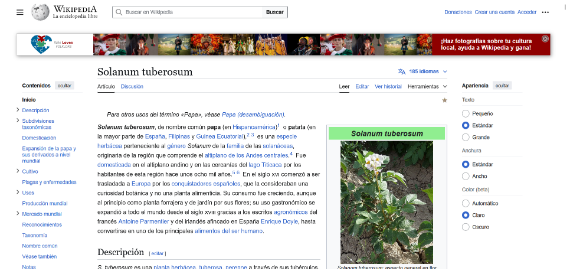
\includegraphics[width=0.8\textwidth]{figures/patata_claro.png}
    \caption{Wikipedia page about potatoes in positive display polarity\cite{patata}}
    \label{fig:patata_claro}
\end{figure}
\begin{figure}
    \centering
    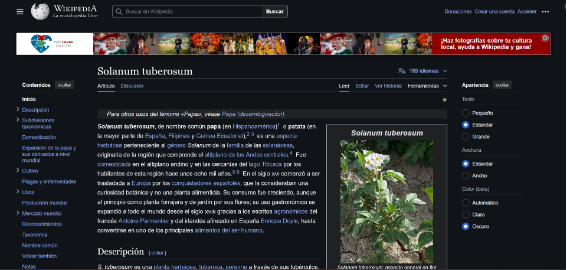
\includegraphics[width=0.8\textwidth]{figures/patata_oscuro.png}
    \caption{Wikipedia page about potatoes in negative display polarity\cite{patata}}
    \label{fig:patata_oscuro}
\end{figure}

\subsubsection{Amazon product}
\begin{figure}
    \centering
    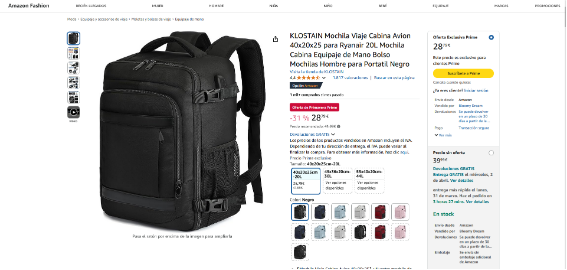
\includegraphics[width=0.8\textwidth]{figures/mochila_claro.png}
    \caption{Amazon product page in positive display polarity\cite{mochila}}
    \label{fig:amazon_claro}
\end{figure}
\begin{figure}
    \centering
    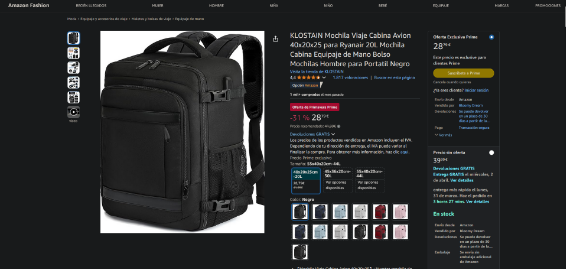
\includegraphics[width=0.8\textwidth]{figures/mochila_oscuro.png}
    \caption{Amazon product page in negative display polarity\cite{mochila}}
    \label{fig:amazon_oscuro}
\end{figure}
\subsection{Final Questionnaire}